\section{Implementation}
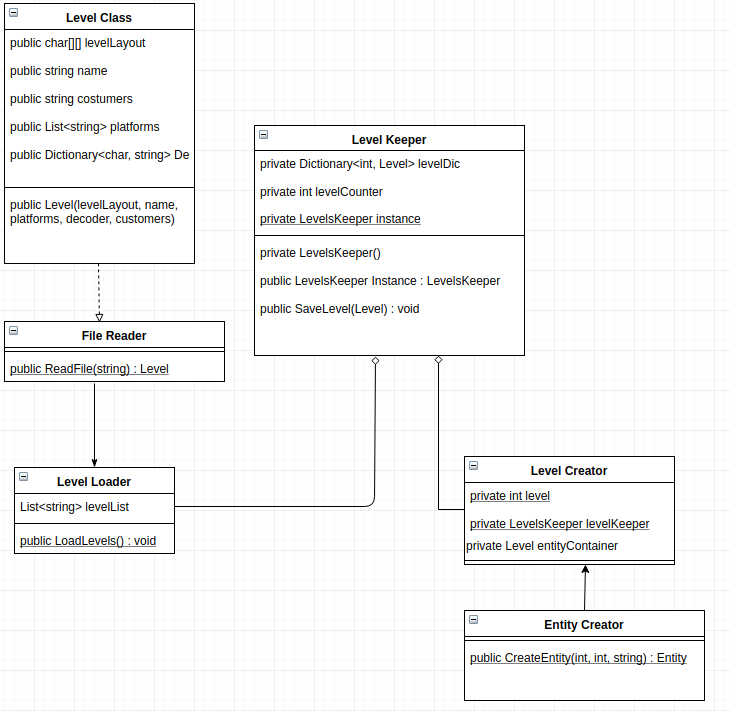
\includegraphics[width=\linewidth]{latex/Images/UML.png}

Som det ses på vores class diagram så er de fleste af vores klasser statiske. Da vi ikke skal bruge flere instanser af for eksempel LevelLoader så vi det mere intuitivt at holde Program og Game fri for objekter som kun skal benyttes en eller få gange, og i stedet bare lade dem kalde statiske metoder i de statiske klasser.\\
Undtagelser på det ovenstående er vores Level class som instatierer et nyt Level objekt. Da vi ønsker at benytte vores Level objekter som en måde at lagre information om vores levels, har vi valgt kun at implementere en konstruktor til dem og ellers gemme alle informationer i public properties uden setters. Dette garanterer at når Level først er blevet instantieret kan dens informationer ikke overskrives, men informationerne kan til enhver tid læses.\\
En anden undtagelse er LevelsKeeper. LevelsKeeper fungerer som en database for vores levels, og indeholder en dictionary af level numre som keys og Level objekter som values. LevelsKeeper er implementeret som en singleton. Dette er gjort da vi ikke ønsker at have flere 'halve' databaser med kun en delmængde af vores levels. Vi vil dog have et problem hvis der skrives og læses til det samme sted i hukommelsen samtidigt da vi arbejder med referencer. Men som det fremgik af vores sequence diagram vil dette ikke kunne lade sig gøre med den nuværende implementation, men skulle det blive nødvendigt at udvide vores model med endnu en klasse som skriver til LevelsKeeper samtidigt med at spillet kører, så så skal der implementeres en form for sikkerhed imod dette.\\
At LevelsKeeper er en singleton bevirker at både LevelLoader og LevelCreator skal holde en variabel for LevelsKeeper objektet, som kan kalde sin private metode til at gemme et Level objekt, eller kan benytte sin public property til at returnere et level hvis den er givet et indeks. Metoden er privat, og propertien har ingen setter for at følge princippet om at hver class udfører opgaverne for sit eget ansvar.\\

I LevelCreator har vi en liste af EntityContainers som er ment til at holde henholdsvis blokke og platforme. I LevelCreator laver vi et tjek for om den karakter som vi ønsker at lave om til en entity er en blok eller en platform. Der gøres dernæst et kald til EntityCreator som returnere vores entity og LevelCreator indsætter denne entity i den korrekte EntityContainer. Årsagen til denne implementation skyldes at vi i GameRunning (som får givet denne liste af EntityContainers) gerne vil kunne skelne mellem platforme og blokke. Vi kan derfor (i GameRunning) når der udføres collision detection først iterere over listen af blokke, og hvis der her er en collision slutte spillet. Ellers efterfølgende iterere over listen af platforme, og hvis der er en collision her, så ved vi at det er en platform og vi kan gøre vores tjek for hastighed og retning.\\

En væsentlig del af SpaceTaxi er fysikken i spillet. Denne har vi valgt at integrere med spilleren da vi ved at der ikke vil være andre objekter som skal benytte den. Vi vælger altså at se fysikken i spillet som den måde spilleren skal bevæge sig på, og der er derfor stadig player objektets ansvar at kunne bevæge sig korrekt.\\
Vi har implementeret tyngdekraften således at vi kan tænde og slukke den. Dette skyldes at når spilleren lander på en platform, så ønsker vi ikke at den skal falde igennem platformen. Derfor slukker vi for tyngdekraften og spillerens fart sættes til nul (forudsat at den ikke dør på grund af en for hård landing eller dårlig vinkel). Tyngdekraften tændes dernæst først igen når rumskibet letter fra platformen. Vi oplever dog at rumskibet kan falde igennem platforme hvis den laver små hop. Vi mistænker dette skyldes at der ikke bliver foretaget collision detection hvis rumskibet bevæger sig meget langsomt, men det er ikke lykkedes os verificere dette.